\documentclass[10pt]{article}
\usepackage{../../local}
\urlstyle{same}

\newcommand{\classcode}{EE 120}
\newcommand{\classname}{Signals and Systems}
\renewcommand{\maketitle}{%
\hrule height4pt
\large{Eric Du \hfill \classcode}
\newline
\large{HW 06} \Large{\hfill \classname \hfill} \large{\today}
\hrule height4pt \vskip .7em
\small{Header styling inspired by CS 70: \url{https://www.eecs70.org/}}
\normalsize
}
\linespread{1.1}
\renewcommand{\familydefault}{\sfdefault}
\begin{document}
	\maketitle
	\section*{Collaborators}
	I worked with the following people on this assignment:
	\begin{itemize}
		\item Teja Nivarthi: 3036508567
		\item Nikhil Maserang: 3036978230
	\end{itemize}
	\section*{Problem 1}
	A Vandermonde matrix is a \( (m +1 ) \times (m +1) \) matrix of the form
	\[
		V = \begin{bmatrix} 1 & x_0 & x_0^2 & \dots & x_0^{m}\\ 1 & x_1 & x_1^2 & \dots & x_1^{m}\\
		\vdots & \vdots & \vdots & \ddots & \vdots \\
	1 & x_m & x_m^2 & \dots & x_m^{m}\end{bmatrix} 
	\] 
	for some complex numbers \( x_0, x_1, \dots, x_m \). A Vandermonde matrix always has determinant:
	\[
	\det V = \prod_{j = 1}^{m}\prod_{i = 0}^{j - 1}(x_j - x_i)
	\] 
	\begin{enumerate}[label=\alph*), start]
		\item Show that \( V  \) is invertible if and only if no two  \( x_i \) are the same.

			\begin{solution}
				We know from linear algebra that a matrix is invertible if and only if the determinant 
				is nonzero. Consequently, this is also only true if no two \( x_i \)'s are the same, since the 
				above formula for the determinant shows us that the determinant would be zero if that were the case.
			\end{solution}
	\end{enumerate}
	We can use \( V \) to perform \textbf{polynomial interpolation}. In particular, consider a degree at 
	most \( m \) polynomial \( p(x) = a_0 + a_1x + \cdots + a_{m - 1}x^{m - 1} + a_m x^{m} \). We do not 
	know the \( a_j \), but we have pairs \( (x_j, y_j) \) for \( j = 0 \) to \( m \) such that 
	\( y_j = p(x_j) \). 
	\begin{enumerate}[label=\alph*), resume]
		\item Write a matrix-vector equation which allows one to recover
			\[
				a := \begin{bmatrix} a_0\\a_1\\ \vdots \\ a_m \end{bmatrix} 
				\ \text{from} \ y:= \begin{bmatrix} y_0\\y_1\\ \vdots \\ y_m \end{bmatrix} 
			\] 
			 as long as the  \( x_j \) 's are not equal. 

			 \begin{solution}
				We know that based on the vector equation, that \( y = Va \), so in order to determine \( a \), 
				then we multiply both sides by \( V^{-1} \) on the left:
				\[
				a = V^{-1} y
				\] 
				Again, this requres that \( V \) is invertible, which is guaranteed as long as the \( x_j \)'s are 
				not equal.
			 \end{solution}
	\end{enumerate}
	For the next subpart, assume we use the DFT matrix formulation:
	\[
		\vec x = \begin{bmatrix} x[0]\\x[1]\\ \vdots \\x[N-1] \end{bmatrix} \quad 
		\vec X = \begin{bmatrix} X[0] \\ X[1] \\ \vdots \\ X[N-1] \end{bmatrix} \quad
		\mathbf F = \begin{bmatrix} e^{-j \frac{2\pi}{N} 0 \cdot 0} & e^{-j \frac{2\pi}{N} 1 \cdot 0 }
		& \cdots & e^{-j \frac{2\pi}{N}N \cdot 0}\\ e^{-j \frac{2\pi}{N} 0 \cdot 1} & 
		e^{-j \frac{2\pi}{N} 1 \cdot 1} & \cdots & e^{-j \frac{2\pi}{N}N \cdot 1}\\
	\vdots & \vdots & \ddots & \vdots \\
	e^{-j \frac{2\pi}{N} 0 \cdot N} & e^{-j \frac{2\pi}{N} 1 \cdot N} & \cdots & e^{-j \frac{2\pi}{N}N \cdot N}
	\end{bmatrix} 
	\] 
	where \( \vec X = \mathbf F \vec x \)
	%By uniqueness, this means that there is only one degree at most \( m \) polynomial going through 
	%\( m+1 \) different points.
	\begin{enumerate}[label=\alph*), resume]
		\item The DFT matrix for an \( (m+1) \)-length signal \( z[n] \) where \( z[n] = 0 \) outside 
			the interval \( 0 \le n \le m \) is actually a Vandermonde matrix. Show this by picking suitable 
			values for \( x_0, x_1, \dots, x_m \). This gives us another interpretation of DFT: it transforms 
			polynomials to their evaluations on this set of points.

			\begin{solution}
				Looking at the matrix \( \mathbf F \), we can see that in each row, we have one of the \( N \) 
				roots of unity, then along the row we exponentiate it from 1 to \( N \). Therefore, one way 
				we can pick \( x_0, \dots, x_m \) is:
				\[
				x_k = e^{-j \frac{2\pi}{N} k} = \omega_1^{k}
				\] 
				where \(  \omega_1 \) is the first nontrivial \( N \)-th root of unity.
			\end{solution}
	\end{enumerate}
	\pagebreak
	\section*{Problem 2}
	Find the CTFT \( X(\omega) \) of \( x(t) \), where 
	\[
		\forall t \in \R, x(t) = \frac{1}{\sigma\sqrt{2\pi} }\exp{-\frac{t^2}{2\sigma^2}}
	\] 
	and \( \sigma > 0 \). You may or may not find it useful to know that 
	\begin{enumerate}[label=\roman*)]
		\item \( \int_{-\infty}^{\infty} x(t) \diff t  = 1 \) 
		\item \( \int_{a}^{b} u \diff v = uv\biggr|_a^{b} - \int_{a}^{b} v \diff u   \) 
		\item \( tg(t) \leftrightarrow i \dv{G(\omega)}{\omega} \)
		\item \( \int_{0}^{\omega} \frac{1}{G(\lambda)}\dv{G(\lambda)}{\lambda} = \ln G(\omega)\biggr|_0^{\omega}  \)
	\end{enumerate}
	\textit{Hint:} Take the derivative of the given equation for \( x(t) \) and use CTFT properties and the above hints
	to take the Fourier transform of both sides. 

	\begin{solution}
		First, we can write out the Fourier transform:
		\[
		X(\omega) = \frac{1}{\sigma \sqrt{2\pi} }\int_{-\infty}^{\infty} e^{-(t^2 / 2 \sigma^2 + i \omega t)}
		\diff t
		\] 
		To continue doing this integral, I prove the following relation first:
		\[
		\int_{-\infty}^{\infty} e^{-\frac{a}{2}x^2 + bx} = e^{\frac{b^2}{2a}}\sqrt{\frac{2\pi }{a}} 
		\] 
		First, we factor out \( -\frac{a}{2} \) from the exponent:
				\[
					I = \iinf e^{-\frac{a}{2}(x^2 + \frac{2b}{a}x)} dx
				\] 
		And now we complete the square:
		\[
			I = \iinf e^{-\frac{a}{2}\left(\left(x - \frac{b}{a}\right)^2 - \frac{b^2}{a^2}\right)} dx
			= \iinf e^{-\frac{a}{2}\left( x - \frac{b}{a} \right)^2 + \frac{b^2}{2a}} dx = e^{\frac{b^2}{2a}}
			\iinf e^{-\frac{a}{2}\left( x - \frac{b}{a} \right)^2} dx
		\] 
		Now we perform a \( u \)-substitution \( u = x + \frac{b}{a} \) so \( du = dx \), therefore:
		\[
			I = e^{\frac{b^2}{2a}} \iinf e^{-\frac{a}{2}u^2} du
		\] 
		Now perform a second substitution \( r = \sqrt{\frac{a}{2}}u \), so therefore \( r^2 = \frac{a}{2}u^2 \):
		\begin{equation}\label{eq1}
		I = \sqrt{\frac{2}{a}}e^{\frac{b^2}{2a}}\int_{-\infty}^{\infty} e^{-r^2} \diff r 
		\end{equation} 
		It's a well known result that the remaining integral simplifies to \( \sqrt{\pi}  \), but I'll prove 
		it as well. I'll use \( x \) instead of \( r \), since we're going to use that later. First, we calculate 
		the square of the integral:
		\[
			I'^2 = \left( \int_{-\infty}^{\infty} e^{-x^2} \diff x  \right) \left( \int_{-\infty}^{\infty} 
			e^{-y^2} \diff y\right) = \int_{-\infty}^{\infty} \int_{-\infty}^{\infty} e^{-(x^2 + y^2)} \diff x \diff y  
		\] 
		We know that \( x^2 + y^2 = r^2 \), and switching this to polar coordinates:
		\[
		I'^2 = \int_{0}^{\infty} \int_{0}^{2\pi} e^{-r^2} r \diff \theta \diff r = \int_{0}^{2\pi} \diff \theta
		\int_{0}^{\infty} e^{-r^2} r \diff r 
		\] 
		The second integral can be solved via a \( u \)-substitution \( u = r^2 \) so \( du = 2r \diff r \), so:
		\[
		I'^2 = 2\pi \frac{1}{2}\int_{0}^{\infty} e^{-u} \diff u 
		\] 
		The integral evaluates to 1 (I'm just too lazy to show it explicitly at this point), meaning that
		\( I' = \sqrt{\pi}  \) after taking the square root. Returning to the original integral (equation 
		\ref{eq1}), we get: 
		\[
		I = \sqrt{\frac{2\pi}{a}} e^{\frac{b^2}{2a}}
		\] 
		as desired. Now we can finally proceed with our Fourier transform. In the equation, we identify that 
		\( a = \frac{1}{\sigma} \), and \( b = -i \omega \). Therefore, the integral simplifies to:
		\[
			X(\omega) = \frac{1}{\sigma \sqrt{2\pi} }e^{-\omega^2 \sigma^2 / 2}\sqrt{2\pi \sigma^2} 
			= e^{-\omega^2 \sigma^2 / 2}
		\] 
		This is also an expected result: we know in literature that the Fourier transform of a Gaussian 
		is a Gaussian; in fact, it is this property that makes the Gaussian the "minimum uncertainty" wavepacket 
		between position and momentum in quantum mechanics. 
		I imagine it to work the exact the same between temporal support
		and the bandwidth in frequency space since both things (position/momentum vs. frequency/time) are related
		by a simple Fourier transform.
	\end{solution}
	\pagebreak
	\section*{Problem 3} 
	Consider a discrete-time signal \( x: \Z \to \C \) that has a Fourier transform (DTFT) \( X: \R \to \C \). 
	\begin{enumerate}[label=\alph*)]
		\item Let \( \hat X\) be such that 
			\[
				\forall \omega \in \R, \quad \hat{X}(e^{j \omega}) = j\dv{X}{\omega}(e^{j \omega})
			\]
			Determine an expression for \( \hat{x}(n) \). 

			\begin{solution}
				Using the definition for the derivative property:
				\[
					nx[n] \quad \leftrightarrow j \dv{X(e^{j \omega})}{\omega} 
				\] 
				since the right hand side of this is what we have for \( \hat{X}e^{j \omega}) \), then it means 
				that \( \hat{x}[n] \) must correspond to the left hand side. This means that:
				\[
					\hat{x}[n] = nx[n]
				\] 
			\end{solution}
		\item Let \( \hat{x} \) be such that 
			\[
				\forall n \in \Z, \quad \hat{x}[n] = \begin{cases}
					x\left( \frac{n}{N} \right)  & \text{if \( n \) mod \( N = 0\)}\\
					0 & \text{otherwise}
				\end{cases}
			\] 
			for some integer \( N \).
			\begin{enumerate}[label=\roman*)]
				\item Show that \( \hat{X} \), the DTFT of \( \hat{x} \), is
					\[
					\forall \omega \in \R, \quad \hat{X}(e^{j \omega}) = X(e^{j N \omega})
					\] 

					\begin{solution}
						The proof of this was covered in lecture: let's take the Fourier transform of 
						\( \hat{x}[n] \):
						\begin{align*}
							\sum_{n=-\infty}^{\infty} \hat{x}[n]e^{- j \omega n } &= \sum_{k=-\infty}^{\infty} x[kN]
							e^{-j \omega kN}\\
							&= \sum_{k=-\infty}^{\infty} x[k]e^{-j (N\omega) k}\\
							&= X(e^{j N \omega}) 
						\end{align*}	
						as desired. 
					\end{solution}
				\item Consider the causal echo system characterized by the linear, constant-coefficient difference
					equation
					\[
						\hat{y}[n] = \hat{x}[n] + \alpha \hat{y}[n - N]
					\] 
					where \( |\alpha| < 1 \) and \( \hat{x} \) and \( \hat{y} \) denote the input, and output, 
					respectively. Show that the frequency response \( \hat{H} \) of this system is 
					\[
						\forall \omega \in \R, \hat{H}(e^{ j \omega}) = \frac{1}{1 - \alpha e^{-i \omega N}}
					\] 

					\begin{solution}
						Recall that to compute frequency response, we let \( \hat{x}[n] = Ae^{i \omega n} \), 
						and \( \hat{y}[n] = H(\omega) Ae^{j \omega n} \). Therefore:
						\[
						\hat{H}(\omega)Ae^{i \omega n} = Ae^{i \omega n} + \alpha \hat{H}(\omega)e^{i \omega (n - N)}
						\] 
						dividing both sides by \( Ae^{i \omega n} \) and collecting \( \hat{H}(\omega) \), we get:
						\[
							\hat{H}(\omega) = \frac{1}{1 - \alpha e^{- i \omega N}}
						\] 
						as desired. 
					\end{solution}
				\item How is \( \hat{H} \) related to the frequency response \( H \) of the causal system 
					described by the linear, constant-coefficient difference equation
					\[
						y[n] = x[n] + \alpha y[n - 1]
					\] 
					where \( |\alpha| < 1 \), and \( x \) and \( y \) denote the input and output, respectively?

					\begin{solution}
						This system is the special case where \( N = 1 \), so therefore we have:
						\[
						H(\omega) = \frac{1}{1 - \alpha e^{-i \omega}}
						\] 
						So in terms of input, we have \( H(\omega N) = \hat{H}(\omega) \). 
					\end{solution}
				\item Determine the impulse response values \( h[n], \forall n\in \Z\). Then use the up-sampling 
					property to determine the sample values of the impulse response \( \hat{h}[n] \).

					\begin{solution}
						Solving the LCCDE from the previous part, we have:
						\[
							y[n] = \sum_{k=0}^{n} \alpha^{n-k}x[k]
						\] 
						Therefore, the impulse response \( h[n]\) is given by feeding in \( x[k] = \delta[k] \):
						\[
							h[n] = \sum_{k=0}^{n} \alpha ^{n - k}\delta[k] = \alpha ^{n}u[n + N]
						\] 
						where the last equality comes from noticing that for every \( n \), there is only  
						one term in this sum that is nonzero, which is the delta function with \( \alpha ^{k}\) 
						attached to it. We then have a step function to enforce that values above 
						\( n \) are zeroed out. 
						Then, using the up-sampling property, we know that \( \hat{h}[n] = h[\frac{n}{N}] \):
						\[
							\hat{h}[n] = \sum_{k=0}^{n / N} \alpha ^{n / N} u[n / N + N]
						\] 
					\end{solution}
			\end{enumerate}
	\end{enumerate}
	\pagebreak
	\section*{Problem 4} 
	Consider a \textit{\textbf{real-valued}, causal} discrete-time signal \( x \) and its 
	Fourier transform \( X \). The real part of the signal's Fourier transform is given by 
	\[
	\Re \{X(e^{j \omega})\}  = 1 + \cos(\omega) - \cos(2 \omega)
	\] 
	On midterm 1, we derived \( X(e^{j \omega}) \) by splitting it up into its real and imaginary parts. Now, we use 
	DTFT properties! :)
	\begin{enumerate}[label=\alph*)]
		\item Using DTFT properties, evaluate the integral \( \int_{\mean{2\pi}} X(e^{ j \omega}) \diff \omega \).

			\begin{solution}
				This is basically an exercise in rewriting an integral: 
				\begin{align*}
				\int_{\mean{2\pi}} \Re \{X(e^{ j \omega}\} \diff \omega &= \int_{\mean{2\pi}} \frac{1}{2}
				(X(e^{j \omega}) + X^{*}(e^{j \omega})) \diff  \omega\\
				&= \frac{1}{2}\int_{\mean{2\pi}} X(e^{j \omega}) \diff \omega + 
				\frac{1}{2} \int_{\mean{2\pi}} X^{*}(e^{j \omega}) \diff \omega
			\end{align*}
			Since \( x[n] \) is real-valued, then we know that \( X^{*}(e^{j \omega}) = X(e^{- j \omega}) \), 
			which we can now write as:
			\[
				\int_{\mean{2\pi}} \Re \{X(e^{ j \omega})\} \diff  \omega = 
				\frac{1}{2}\int_{\mean{2\pi}} X(e^{ j \omega}) \diff \omega + \frac{1}{2}
				\int_{\mean{2\pi}} X(e^{j (- \omega)}) \diff  \omega
			\] 
			So this means that if we pick a suitable (odd) interval \( \omega \in [-\pi, \pi] \), then the two 
			integrals are both identical, therefore, we have:
			\[
			\int_{-\pi}^{\pi} \Re \{X(e^{j \omega})\} \diff \omega  = \int_{-\pi}^{\pi} X(e^{j \omega}) \diff \omega 
			\] 
			Computing the left hand side since we're given \( \Re \{X(e^{j \omega})\} \), we get:
			\[
			\int_{-\pi}^{\pi} X(e^{j \omega}) = 2\pi 
			\] 
			It then follows from the fact that the exponentials along any interval of width \( 2\pi \) is periodic 
			that:
			\[
				\int_{\mean{2\pi}}X(e^{j \omega}) \diff \omega= 2\pi
			\] 
			\end{solution}
		\item Determine, and provide a well-labeled plot of the signal \( x \).

			\begin{solution}
				From the earlier part, because we've shown that computing the integral for 
				\( \Re \{X(e^{j \omega})\} \) 
				is the same as computing the integral for the total \( X(e^{j \omega}) \), 
				 this implies that 
				 \[
				 \Re \{X(e^{j \omega})\}  = X(e^{j \omega})
				 \] 
				 Therefore, now we can just find \( x[n] \) via the DTFT synthesis equation:
				 \[
					 x[n] = \frac{1}{2\pi}\int_{\mean{2\pi}} X(e^{j \omega}) e^{j \omega n }\diff \omega
					 = \frac{1}{2\pi}\int_{\mean{2\pi}} (1 + \cos \omega - \cos(2 \omega)) e^{j \omega n}
					 \diff \omega
				 \] 
				 This evaluates to:
				 \[
					 x[n] = \frac{1}{2}(-\delta[n - 2] + \delta[n - 1] + 2 \delta[n] + \delta[n + 1] - \delta[n + 2])
				 \] 
				 As for the plot, we've done this a million times but here's how I understand it: at \( n = \pm 2 \), 
				 we have peaks of \( -\frac{1}{2} \), at \( n = \pm 1 \) we have peaks of \( \frac{1}{2} \), and 
				 at \( n = 0 \) we have a peak of 1 because we have \( 2 \delta[n] \) which cancels out the 
				 prefactor of \( \frac{1}{2} \). For all other \( n \), we have \( x[n] = 0 \). 
				 I'm explaining it like this to show that I do understand how to 
				 plot functions like these; I am simply using Mathematica becuase it takes less time: 
				 \begin{center}
					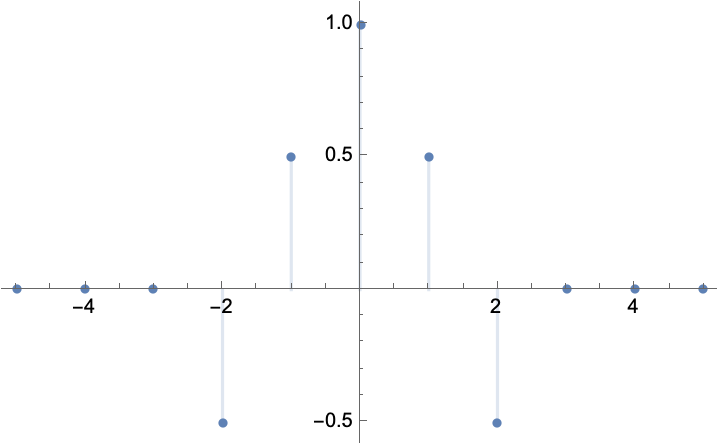
\includegraphics[scale=0.8]{q4b.png}	
				 \end{center}
			\end{solution}
		\item Evaluate the integral \( \int_{\mean{2\pi}} X(e^{j \omega})\cos(\omega) \diff \omega \).

			\begin{solution}
				Written out, we're basically asked to compute:
				\[
					\int_{\mean{2\pi}}(1 + \cos \omega - \cos(2 \omega)) \cos \omega \diff \omega 
					= \int_{0}^{2\pi} \cos \omega \diff \omega + \int_{0}^{2\pi} \cos^2 \omega \diff  \omega
					- \int_{0}^{2\pi} \cos \omega \cos(2 \omega) \diff \omega 
				\] 
				We can notice that the first and third integrals evaluate to zero (since we're integrating 
				a cosine wave over its entire period), so we're left with the second integral:
				\begin{align*}
					\int_{0}^{2\pi} \cos^2  \omega \diff \omega &= \int_{0}^{2\pi} \frac{1 + \cos(2\omega)}{2}\diff 
					\omega\\
					&= \left[ \frac{\omega}{2} + \frac{1}{4}\sin(2 \omega) \right]_0^{2\pi}\\
					&= \pi 
				\end{align*}
				Therefore, we conclude:
				\[
					\int_{\mean{2\pi}} X(e^{j \omega}) \diff \omega = \pi
				\] 
			\end{solution}
		\item Evaluate the integral 
			\[
				\int_{\mean{2\pi}}|X(e^{j \omega})|^2 \diff  \omega
			\] 

			\begin{solution}
				Well, we know that \( X(e^{j \omega}) = \Re \{S(e^{ j \omega}\}  \), so basically we just have to 
				compute:
				\[
					\int_{\mean{2\pi}}|1 + \cos(\omega) - \cos(2 \omega)|^2 \diff \omega
				\] 
				We can use Parseval's theorem to massively simplify our life, which states:
				\[
				\frac{1}{2\pi}	\int_{\mean{2\pi}}|X(e^{j \omega})|^2 \diff \omega = \sum_n |x[n]|^2
				\]  
				Therefore, we have:
				\[
					\int_{\mean{2\pi}} |X(e^{j \omega})|^2 \diff \omega = \frac{1}{2\pi}
					\left( 1 + 2 * \left( -\frac{1}{2} \right)^2 + 2 * \left( \frac{1}{2} \right)^2 \right) 
					= 4\pi
				\] 
			\end{solution}
		\item Determine a reasonably simple expression for \( \Im \{X(e^{j \omega}) \}  \), the imaginary part of the 
			signal's Fourier transform, where, as you know, 
			\[
			X(\omega) = \Re \{X(e^{ j \omega}) \} + i \Im \{X(e^{j \omega})\} 
			\] 

			\begin{solution}
				We've already concluded earlier in this problem that \( X(e^{j \omega} = \Re \{X(e^{j \omega})\} \), 
				so this would directly imply that \( \Im \{X(e^{j \omega}) \} = 0 \). 

				I'm going to preface by saying that I probably did something wrong in this problem, but I don't have 
				enough time to figure out what that is. 
			\end{solution}
	\end{enumerate}
	\pagebreak
	\section*{Problem 5} 
	Consider a finite impulse response (FIR) filter \( H : [\Z \to \R] \to [\Z \to \R]\) having impulse 
	response \( h \) and frequency response \( H \). 

	Part (a) below discloses several pieces of information about the filter \( H \). Your task in that part 
	is to determine the impulse response \( h \) completely. 

	In the subsequent parts you explore the filter \( h \) of the part (a) further. 

	Suppose you're given the following pieces of information of the filter \( H \):
	\begin{enumerate}[label=\Roman*)]
		\item \( H \) is a causal filter
		\item There exists a filter \( \text{A}: [\Z \to \R] \to [\Z \to \R] \) having impulse response \( a \) and 
			frequency response \( A \), about which we know the following:
			\begin{enumerate}[label=\roman*)]
				\item \( \forall \omega \in \R, A(e^{j \omega}) = H(e^{j \omega}) e^{j 2 \omega} \).
				\item \( \int_{\mean{2\pi}} A(e^{ j \omega}) \diff \omega = 12\pi \), where 
					\( \mean{2\pi} = [0, 2\pi], [-\pi, \pi] \), or another continuous interval of length 
					\( 2\pi \). 
				\item \( \forall \omega \in \R, A(e^{j \omega}) \in \R\)
				\item The figure below depicts \( A(e^{j \omega}), \forall \omega \in [-\pi, +\pi] \). 
					\begin{center}
						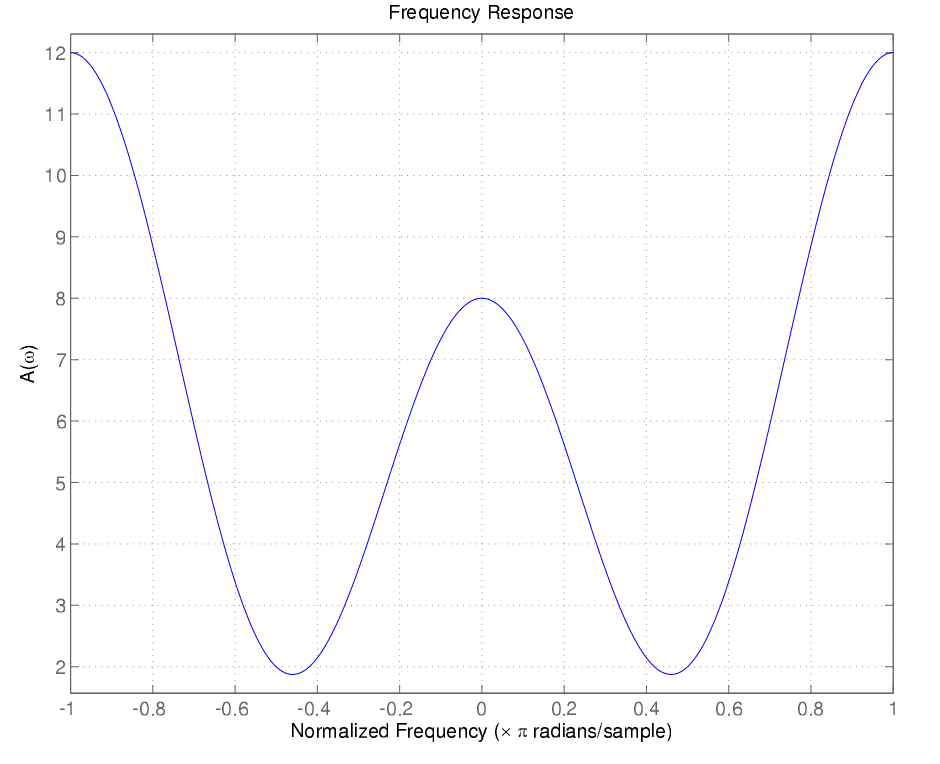
\includegraphics[scale=0.65]{q5.png}
					\end{center}
			\end{enumerate}
	\end{enumerate}

	\begin{enumerate}[label=\alph*)]
		\item Determine, and provide a well-labeled plot of, the impulse response \( h \). 

			\begin{solution}
				From the frequency shift property:
				\[
				x(t - t_0) = e^{j \omega t_0}X(\omega)
				\] 
				This means that \( a[n] = h[n + 2] \), since we've picked up a phase of \( e^{2 i \omega} \). Then, 
				condition (iii) says that \( A \) is real-valued, and the plot for condition (iv) shows us 
				that  \( A \) is also even, meaning that the filter \( a \) is also real-valued and 
				even. 

				We also know that \( H \) is a causal filter, so this means that since \( a[n] = h[n + 2] \) 
				this implies that \( a[n] = 0 \) for all \( n < -2 \). Combining this with the fact that \( a[n] \) 
				is even, this implies that \( a[n] = 0\) for all \( n > 2 \) as well. 

				Now, we look at the plot of \( A(e^{j \omega}) \) in order to figure out the values of \( a \). Recall
				the synthesis equation:
				\[
					A(e^{j \omega}) = \sum_{n=-\infty}^{\infty} a[n] e^{- j \omega n }
				\] 
				since \( a[n] = 0  \) outside of \( [-2, 2] \), we can restrict our interval:
				\[
					A(e^{j \omega}) = \sum_{n=-2}^{2} a[n] e^{-j \omega n}
				\] 
				Now, since \( a[n] \) is even, we only have to calculate three equations. To do this, let's first
				pick \( \omega = 0 \): 
				\[
					A(\omega =0) = a[0] + 2a[1] + 2a[2] = 8
				\] 
				At \( \omega = \pi \), we have:
				\[
					A(\omega = \pi) = a[-2]e^{2 \pi j} + a[-1] e^{\pi j} + a[0] 
					+ a[1]e^{- \pi j} + a[2] e^{-2 \pi j} = a[0] - 2a[1] + 2a[2] = 12
				\] 
				Finally, to get our third equation, we use the fact that 
				\[
					\frac{1}{2\pi}\int_{\mean{2\pi}} A(\omega) \diff \omega = a[0] = \frac{12\pi}{2\pi} = 6
				\] 
				Therefore, solving for \( a[1] \) and \( a[2] \), we get:
				\[
					a[1] = -1 \quad a[2] = 2
				\] 
				Therefore, with \( a \) determined, we can determine \( h \) using the fact that 
				\( a[n] = h[n + 2] \). We know that since \( a[-2] = a[2] \), this implies that 
				\( h[0] = h[4] = a[2] \), and \( a[-1] = a[1] \) implies that \( h[1] = h[3] = -1\). Finally, 
				\( h[2] = a[0] = 6 \).
				Therefore, the plot of \( h[n] \) is as follows (done in mathematica because it looks nicer 
				than my iPad drawings):
				\begin{center}
					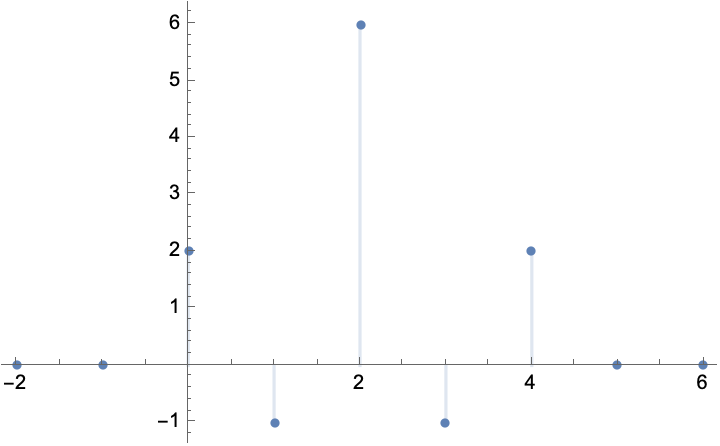
\includegraphics[scale=0.8]{q5a.png}
				\end{center}

			\end{solution}
		\item Let \( x \) be the input and \( y \) the corresponding output of the FIR filter \( H \). 
			Determine the linear, constant-coefficient difference equation governing the input-output 
			behavior of the filter. 

			\begin{solution}
				Here, we just have to write \( h[n] \) in terms of delta functions. With the ceofficients 
				we have from earlier, we can conclude that:
				\[
					h[n] = 2\delta[n] - \delta[n - 1] + 6\delta[n - 2] - \delta[n - 3] + 2\delta[n - 4]
				\] 
				To find \( y[n] \), we just have to turn all the deltas into \( x \):
				\[
					y[n] = 6x[n] - x[n-1] + 6x[n -2] - x[n - 3] + 2x[n - 4]
				\] 
			\end{solution}
		\item Show -- by providing a delay-adder-gain (DAG) block diagram -- how you would implement the filter 
			using a minimal number of delay elements and scalar multiplications. 

			\begin{solution}
				Image below:
				\begin{center}
					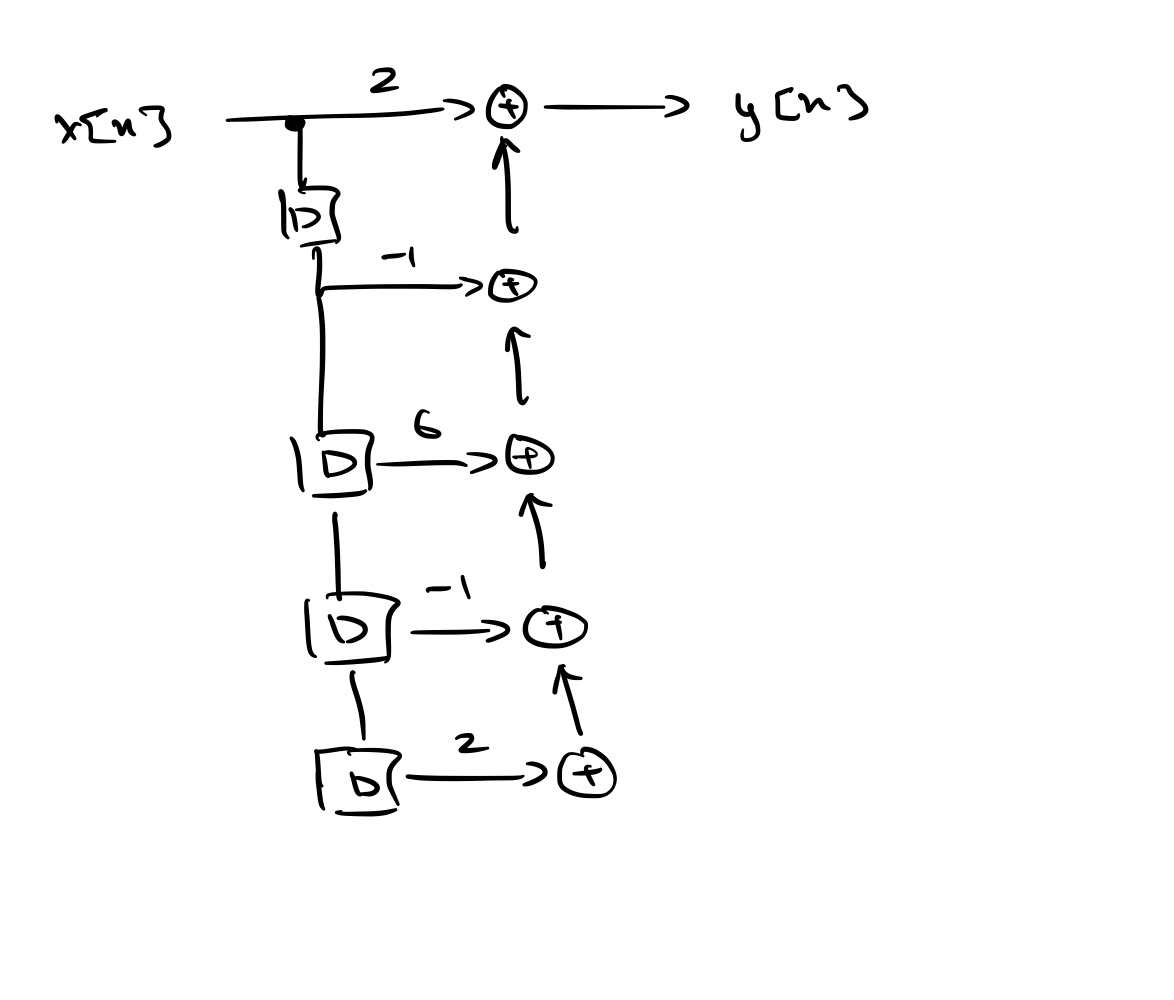
\includegraphics[scale=0.3]{q5c.jpeg}
				\end{center}
			\end{solution}
		\item Determine an expression each for the magnitude response \( |H(e^{j \omega})| \) and phase 
			response \( \angle H(e^{j \omega}) \) of the FIR filter. 

			\begin{solution}
				First we find \( H(\omega) \), using the fact that 
				\[
					H(\omega) = \sum_n h[n] e^{-j \omega n } = 2 - e^{j \omega} + 6e^{-2j \omega}
					- e^{- 3 j \omega} + 2e^{-4 j \omega}
				\] 
				Factoring out \( e^{- 2 j \omega} \), we get:
				\begin{align*}
					H(\omega) &=  e^{-2 j \omega}(2e^{2 j \omega} - e^{j \omega} + 6 - e^{- j \omega} + 
					2e^{-2 j \omega} )\\
					&= e^{-2 j \omega}(4 \cos(2 \omega) - 2 \cos \omega + 6) 
				\end{align*}
				Therefore, the magnitude of this equation is everything but the prefactor:
				\[
				|H(e^{j \omega})| = 4\cos(2 \omega) - 2 \cos \omega + 6
				\] 
				The phase is just the prefactor in front:
				\[
					\angle H(\omega) = -2 \omega
				\] 
			\end{solution}
		\item For each of the following output signals \( x \), determine the corresponding output signal \( y \):
			\begin{enumerate}[label=\alph*)]
				\item \( \forall n, \quad x[n] = 1 \).

					\begin{solution}
						Here we'd have \( y[n] = x[n] * h[n] \), so we'd get:
						\[
							y[n] = \sum_k x[k] h[n - k] = \sum_k h[k] = 8
						\] 
					\end{solution}
				\item \( \forall n, \quad x[n] = (-1)^{n} \) 

					\begin{solution}
						Again, we'd have the same thing:
						\[
							y[n] = \sum_k x[k] h[n - k] = \sum_k (-1)^{k}h[n - k] = (-1)^{n} \cdot 12
						\] 
					\end{solution}
				\item \( \forall n \quad x[n] = \cos\left( \frac{\pi}{4} n\right)  \)

					\begin{solution}
						Same thing:
						\[
							y[n] = \sum_k x[k] h[n - k] = \sum_k \cos(\frac{\pi}{4}n)h[n + k]
						\] 
						Unfortunately, I didn't have enough time to completely finish the evaluation. 
					\end{solution}
			\end{enumerate}
	\end{enumerate}
\end{document}
